\documentclass[../../../../main.tex]{subfiles}
\begin{document}

\begin{flushright}
\footnotesize\textit{【自動文字起こし・要確認】}
\end{flushright}

\noindent
\textbf{[解]} (1) $xy$ 座標平面上で、$x$ 軸の正の部分 (原点 $O$ を端点とする半直線) を始線とし、一般角 $\theta$ に対する動径上で $O$ からの距離 $r\, (r>0)$ の点 $P$ の座標を $(x,y)$ とする。そこで $\sin\theta = \frac{y}{r}, \cos\theta = \frac{x}{r}$ と定義する。

\bigskip

\noindent
(2) 2次元ベクトル $\vec{t}_\theta = \begin{pmatrix} \cos\theta \\ \sin\theta \end{pmatrix}$ とする。
正規直交基底 $\vec{e}_1, \vec{e}_2$ を $\alpha$ だけ回転した直交基底 $\vec{p}, \vec{q}$ を考える。つまり、
\[
\begin{cases} 
\cdot \; \vec{p} \text{ は } \vec{e}_1 \text{ を } \alpha \text{ だけ回転したベクトル} \\ 
\cdot \; \vec{q} \text{ は } \vec{e}_2 \quad \text{〃} 
\end{cases}
\]
とすると、(1)から、
\[
\vec{p} = \begin{pmatrix} \cos\alpha \\ \sin\alpha \end{pmatrix}, \quad \vec{q} = \begin{pmatrix} -\sin\alpha \\ \cos\alpha \end{pmatrix} \quad \cdots \textcircled{1}
\]
ただし、$\vec{q}$ の方は、$y$ 軸を $x$ 軸とみなすことで得られる。次に、$\vec{t}_{\alpha+\beta}$ を考える。

\begin{center}
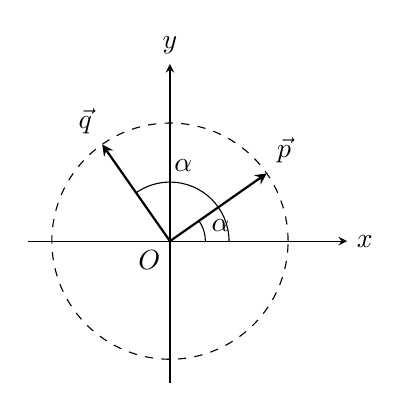
\begin{tikzpicture}[scale=1.5, >=stealth]
  \draw[->] (-1.2, 0) -- (1.5, 0) node[right] {$x$};
  \draw[->] (0, -1.2) -- (0, 1.5) node[above] {$y$};
  \draw[dashed] (0,0) circle (1);
  \node[below left] at (0,0) {$O$};
  \draw[->, thick] (0,0) -- ({cos(35)}, {sin(35)}) node[above right] {$\vec{p}$};
  \draw[->, thick] (0,0) -- ({-sin(35)}, {cos(35)}) node[above left] {$\vec{q}$};
  \draw (0.3, 0) arc (0:35:0.3);
  \node at (17.5:0.45) {$\alpha$};
  \draw (0.5, 0) arc (0:125:0.5);
  \node at (80:0.65) {$\alpha$};
\end{tikzpicture}
\end{center}

これは、$PQ$ 座標からみれば ``$\vec{t}_\beta$'' である。したがって、
\[
\vec{t}_{\alpha+\beta} = \cos\beta \, \vec{p} + \sin\beta \, \vec{q}
\]
成分比較して
\[
\begin{cases} 
\cos(\alpha+\beta) = \cos\beta \cos\alpha - \sin\beta \sin\alpha \\ 
\sin(\alpha+\beta) = \cos\beta \sin\alpha + \sin\beta \cos\alpha 
\end{cases}
\]
を得る。 \hfill $\qed$

\bigskip

\noindent
\[
\cos(\alpha+\beta) = \cos\alpha \cos\beta - \sin\alpha \sin\beta \hfill \text{固}
\]
したがって、
\begin{align*}
\sin(\alpha+\beta) &= \cos\left( \frac{\pi}{2} - (\alpha+\beta) \right) \hfill (*) \\
&= \cos\left\{ \left(\frac{\pi}{2} - \alpha\right) - \beta \right\} \\
&= \cos\left(\frac{\pi}{2} - \alpha\right) \cos(-\beta) - \sin\left(\frac{\pi}{2} - \alpha\right) \sin(-\beta) \\
&= \sin\alpha \cos\beta + \cos\alpha \sin\beta \hfill (*)
\end{align*}

\noindent
又、以下 $(*)$ で用いた変形の証明をする。
\begin{itemize}
  \item[(I)] $\cos(-\alpha) = \cos\alpha, \quad \sin(-\alpha) = -\sin\alpha$ \\
  点 $(\cos(-\alpha), \sin(-\alpha))$ は点 $(\cos\alpha, \sin\alpha)$ と $x$ 軸対称。
  \item[(II)] $\sin\left(\frac{\pi}{2} - \alpha\right) = \cos\alpha, \quad \cos\left(\frac{\pi}{2} - \alpha\right) = \sin\alpha$ \\
  点 $\left(\cos\left(\frac{\pi}{2}-\alpha\right), \sin\left(\frac{\pi}{2}-\alpha\right)\right)$ は点 $(\cos\alpha, \sin\alpha)$ と $x=y$ 対称。
\end{itemize}

\bigskip

\noindent
\textbf{[解2]} (2) $r=1$ として考える。右図で $\vec{OP} = \vec{t}_{\alpha+\beta}$ である。

\begin{center}
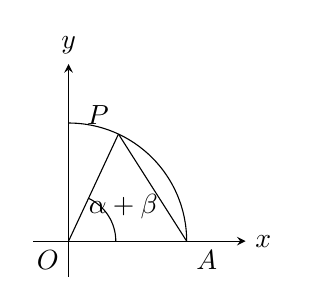
\begin{tikzpicture}[scale=1.5, >=stealth]
  \draw[->] (-0.3, 0) -- (1.5, 0) node[right] {$x$};
  \draw[->] (0, -0.3) -- (0, 1.5) node[above] {$y$};
  \draw (1,0) arc (0:90:1);
  \node[below right] at (1,0) {$A$};
  \node[below left] at (0,0) {$O$};
  \draw (0,0) -- ({cos(65)}, {sin(65)}) node[above left] {$P$};
  \draw (1,0) -- ({cos(65)}, {sin(65)});
  \draw (0.4, 0) arc (0:65:0.4);
  \node at (32.5:0.55) {$\alpha+\beta$};
\end{tikzpicture}
\qquad
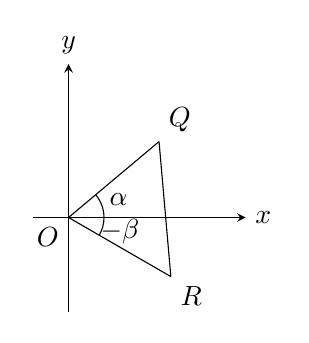
\begin{tikzpicture}[scale=1.5, >=stealth]
  \draw[->] (-0.3, 0) -- (1.5, 0) node[right] {$x$};
  \draw[->] (0, -0.8) -- (0, 1.3) node[above] {$y$};
  \draw (0,0) -- ({cos(40)}, {sin(40)}) node[above right] {$Q$};
  \draw (0,0) -- ({cos(-30)}, {sin(-30)}) node[below right] {$R$};
  \draw ({cos(40)}, {sin(40)}) -- ({cos(-30)}, {sin(-30)});
  \node[below left] at (0,0) {$O$};
  \draw (0.3, 0) arc (0:40:0.3);
  \node at (20:0.45) {$\alpha$};
  \draw (0.3, 0) arc (0:-30:0.3);
  \node at (-15:0.45) {$-\beta$};
\end{tikzpicture}
\end{center}

\noindent
$\cos^2\theta + \sin^2\theta = 1$ に注意して、
\[
|AP|^2 = \{\cos(\alpha+\beta) - 1\}^2 + \sin^2(\alpha+\beta) = 2 - 2\cos(\alpha+\beta) \quad \cdots \textcircled{1}
\]
一方、右図で $\vec{OQ} = \vec{t}_\alpha, \vec{OR} = \vec{t}_{-\beta}$ である。
\[
|QR|^2 = \{\cos\alpha - \cos(-\beta)\}^2 + \{\sin\alpha - \sin(-\beta)\}^2 = 2 - 2(\cos\alpha \cos\beta - \sin\alpha \sin\beta) \quad \cdots \textcircled{2} \hfill (*)
\]
線分 $QR$ を原点まわりに回転すると、線分 $PA$ に重なるので、
\[
|AP|^2 = |QR|^2 \quad \cdots \textcircled{3}
\]
\textcircled{1}～\textcircled{3}から、
\[
\cos(\alpha+\beta) = \cos\alpha \cos\beta - \sin\alpha \sin\beta
\]
\hfill ($\star$高校まではこんなもんで良い。)

\newpage

\end{document}
